\documentclass{article}

\pdfoutput=1

\usepackage[utf8]{inputenc}
\usepackage[T1]{fontenc}
\usepackage[english]{babel}
\usepackage{amsmath}
\usepackage{mathtools}
\usepackage{lmodern}
\usepackage{units}
\usepackage{siunitx}
\usepackage{icomma}
\usepackage{graphicx}
\usepackage{caption}
\usepackage{subcaption}
\usepackage{color}
\newcommand{\N}{\ensuremath{\mathbbm{N}}}
\newcommand{\Z}{\ensuremath{\mathbbm{Z}}}
\newcommand{\Q}{\ensuremath{\mathbbm{Q}}}
\newcommand{\R}{\ensuremath{\mathbbm{R}}}
\newcommand{\C}{\ensuremath{\mathbbm{C}}}
\newcommand{\rd}{\ensuremath{\mathrm{d}}}
\newcommand{\id}{\ensuremath{\,\rd}}
\usepackage{hyperref}
%\usepackage{a4wide} % puts the page numbering further down the page.
\usepackage{pdfpages}
\usepackage{epstopdf}
\DeclareMathOperator{\sgn}{sgn}
\DeclareGraphicsExtensions{.eps}

\title{Home Assigment Week 2}
\author{Marcus Malmquist, marmalm, 941022}
\date{\today}

\begin{document}
\maketitle

\section{Task 1}
The parallel-plate waveguide shown in Figure~\ref{fig:prob} consists of two infinitely wide perfect conductors separated by a distance $d$ and is partially filled with a dielectric, that has a width $W$ and relative permittivity $\epsilon_r=3$, and vacuum everywhere else. The relative permeability is assumed to be $\mu_r=1$ and the electric field strength is assumed to be $E^0_y=|E_y|=\SI{1}{\giga\volt\metre^{-1}}$.
\begin{figure}
  \centering
  \noindent\makebox[\textwidth]{\scalebox{0.9}{\input{problem.pdf_t}}}
  \caption{The figure depicts a parallel-plate waveguide consisting of two infinitely wide perfect conductors separated by a distance $d$ and is partially filled with a dielectric slab that has a width $W$ and vacuum everywhere else.}
  \label{fig:prob}
\end{figure}

\subsection{a}\label{sec:a}
The lowest order TE-mode have the phasor field components seen in (\ref{eq:hz}).
\begin{equation}
  \bar{H}_z(x,y) = 
  \begin{dcases}
    A\sin(K_dx) & \text{, $|x| \leq \frac{W}{2}$} \\
    Be^{-K_a|x|} & \text{, $|x| \geq \frac{W}{2}$} \\
  \end{dcases}
  \label{eq:hz}
\end{equation}
The electric and magnetic field components for a TE-mode can be acquired from (\ref{eq:components}).
\begin{subequations}
  \begin{align}
    \bar{H}_x & = -\frac{\gamma}{h^2}\frac{\partial \bar{H}_z}{\partial x}, \label{eq:hx}\\
    \bar{H}_y & = -\frac{\gamma}{h^2}\frac{\partial \bar{H}_z}{\partial y}, \label{eq:hy}\\
    \bar{E}_x & = -\frac{j\omega\mu}{h^2}\frac{\partial \bar{H}_z}{\partial y}, \label{eq:ex}\\
    \bar{E}_y & = \frac{j\omega\mu}{h^2}\frac{\partial \bar{H}_z}{\partial x}, \label{eq:ey}
  \end{align}
  \label{eq:components}
\end{subequations}
where
\begin{subequations}
  \begin{align}
    \gamma & = \alpha+j\beta, \label{eq:gamma} \\
    h^2 & = \gamma^2+\omega^2\mu\epsilon=
          \begin{dcases}
            h^2_d=K^2_d & \text{, $|x| \leq \frac{W}{2}$} \\
            h^2_a=K^2_a & \text{, $|x| \geq \frac{W}{2}$}
          \end{dcases}, \label{eq:h}
  \end{align}
  \label{eq:values}
\end{subequations}

We can conclude that $\bar{H}_z$ has no $y$-components and we get
\begin{subequations}
  \begin{align}
    \bar{H}_x & =
                \begin{dcases}
                  \frac{\gamma}{h^2}AK_d\cos(K_dx) & \text{, $|x| \leq \frac{W}{2}$} \\
                  \frac{\gamma}{h^2}\sgn(x)BK_ae^{-K_a|x|} & \text{, $|x| \geq \frac{W}{2}$}\end{dcases}, \label{eq:hx2}\\
    \bar{H}_y & = 0 \text{, $\forall x$}, \label{eq:hy2} \\
    \bar{E}_x & = 0 \text{, $\forall x$}, \label{eq:ex2} \\
    \bar{E}_y & = 
                \begin{dcases}
                  \frac{j\omega\mu}{h^2}AK_d\cos(K_dx) & \text{, $|x| \leq \frac{W}{2}$} \\
                  \frac{j\omega\mu}{h^2}\sgn(x)BK_ae^{-K_a|x|} & \text{, $|x| \geq \frac{W}{2}$}\end{dcases} \label{eq:ey2}
  \end{align}
  \label{eq:components2}
\end{subequations}
Knowing that the the the boundary condition for the $H$-field at the interface between vacuum and the dielectric is continous (since there are no free currents), we can relate $\bar{H}_z$ in vacuum to $\bar{H}_z$ in the dielectric since $H_t=H_z$.
\begin{equation}
  A\sin(K_d\frac{W}{2})=Be^{-K_a\frac{W}{2}} \Leftrightarrow B=Ae^{K_a\frac{W}{2}}\sin(K_d\frac{W}{2})
  \label{eq:ab}
\end{equation}
A boundary condition is the $E_x$ and $E_y$ needs to vanish at $y=0$ and $y=d$ but this is already fulfilled since $E_x\equiv 0$ and $E_y\equiv 0$. Another boundary condition is that the normal component of the magetic field and the tangential component of the electric field is continous across an interface, which along with (\ref{eq:ab}) gives
\begin{equation}
  \begin{array}{rcl}
    K_d\cos(K_d\frac{W}{2}) & = & \sgn(x)K_ae^{K_a\frac{W}{2}}\sin(K_d\frac{W}{2})e^{-K_a\frac{W}{2}} \\
     & \\
    \Leftrightarrow \dfrac{K_d}{K_a} & = & \tan(K_d\frac{W}{2})
  \end{array}
  \label{eq:values}
\end{equation}

Since the electric field strength between the two plates is $\SI{1}{\giga\volt\metre^{-1}}$ the amplitude of $\bar{H}_z$ can be related to $E^0_y$.
\begin{equation}
  \dfrac{j\omega\mu}{h^2}AK_d = E^0_y \Leftrightarrow A=-j\dfrac{h^2}{\omega\mu}\dfrac{E^0_y}{K_d}
\end{equation}
This makes the solution for an arbitrary wavelength
\begin{subequations}
  \begin{align}
    \bar{H_z} & =
                \begin{dcases}
                  -j\dfrac{K_d}{\omega\mu}E^0_y\sin(K_dx) & \text{, $|x| \leq \frac{W}{2}$} \\
                  -j\dfrac{K_d}{\omega\mu}E^0_y\sin(K_d\frac{W}{2})e^{-K_a(|x|-\frac{W}{2})} & \text{, $|x| \geq \frac{W}{2}$}
                \end{dcases}, \label{eq:hz_final}\\
    \bar{H}_x & =
                \begin{dcases}
                  -j\dfrac{\gamma}{\omega\mu}E^0_y\cos(K_dx) & \text{, $|x| \leq \frac{W}{2}$} \\
                  -j\sgn(x)\dfrac{\gamma}{\omega\mu}E^0_y\cos(K_d\frac{W}{2})e^{-K_a(|x|-\frac{W}{2})} & \text{, $|x| \geq \frac{W}{2}$}\end{dcases}, \label{eq:hx_final}\\
    \bar{H}_y & = 0 \text{, $\forall x$}, \label{eq:hy_final} \\
    \bar{E}_x & = 0 \text{, $\forall x$}, \label{eq:ex_final} \\
    \bar{E}_y & = 
                \begin{dcases}
                  E^0_y\cos(K_dx) & \text{, $|x| \leq \frac{W}{2}$} \\
                  \sgn(x)E^0_y\cos(K_d\frac{W}{2})e^{-K_a(|x|-\frac{W}{2})} & \text{, $|x| \geq \frac{W}{2}$}\end{dcases} \label{eq:ey_final}
  \end{align}
  \label{eq:components_final}
\end{subequations}

Using (\ref{eq:h}) and (\ref{eq:values}) we can calculated $K_d$ and $K_a$ numerically. The result for the lowest order TE-mode can be seen graphically in Figure~\ref{fig:k_d} and was calculated to $K_d=1690$ which gives $K_a=890$.
\begin{figure}
  \centering
  \noindent\makebox[\textwidth]{\scalebox{0.9}{\input{k_d.pdf_t}}}
  \caption{The figure depicts the numerical solution for $K_d$ at $\SI{30}{\giga\hertz}$.}
  \label{fig:k_d}
\end{figure}

\subsection{b}\label{sec:b}
In the calculations made to plot the intensity for the relevant components a frequency above the cuf-off frequency was used. The chosen frequency was $\SI{50}{\giga\hertz}$ and the width of the dielectric was $\SI{5}{\milli\metre}$
\begin{figure}
  \centering
  \noindent\makebox[\textwidth]{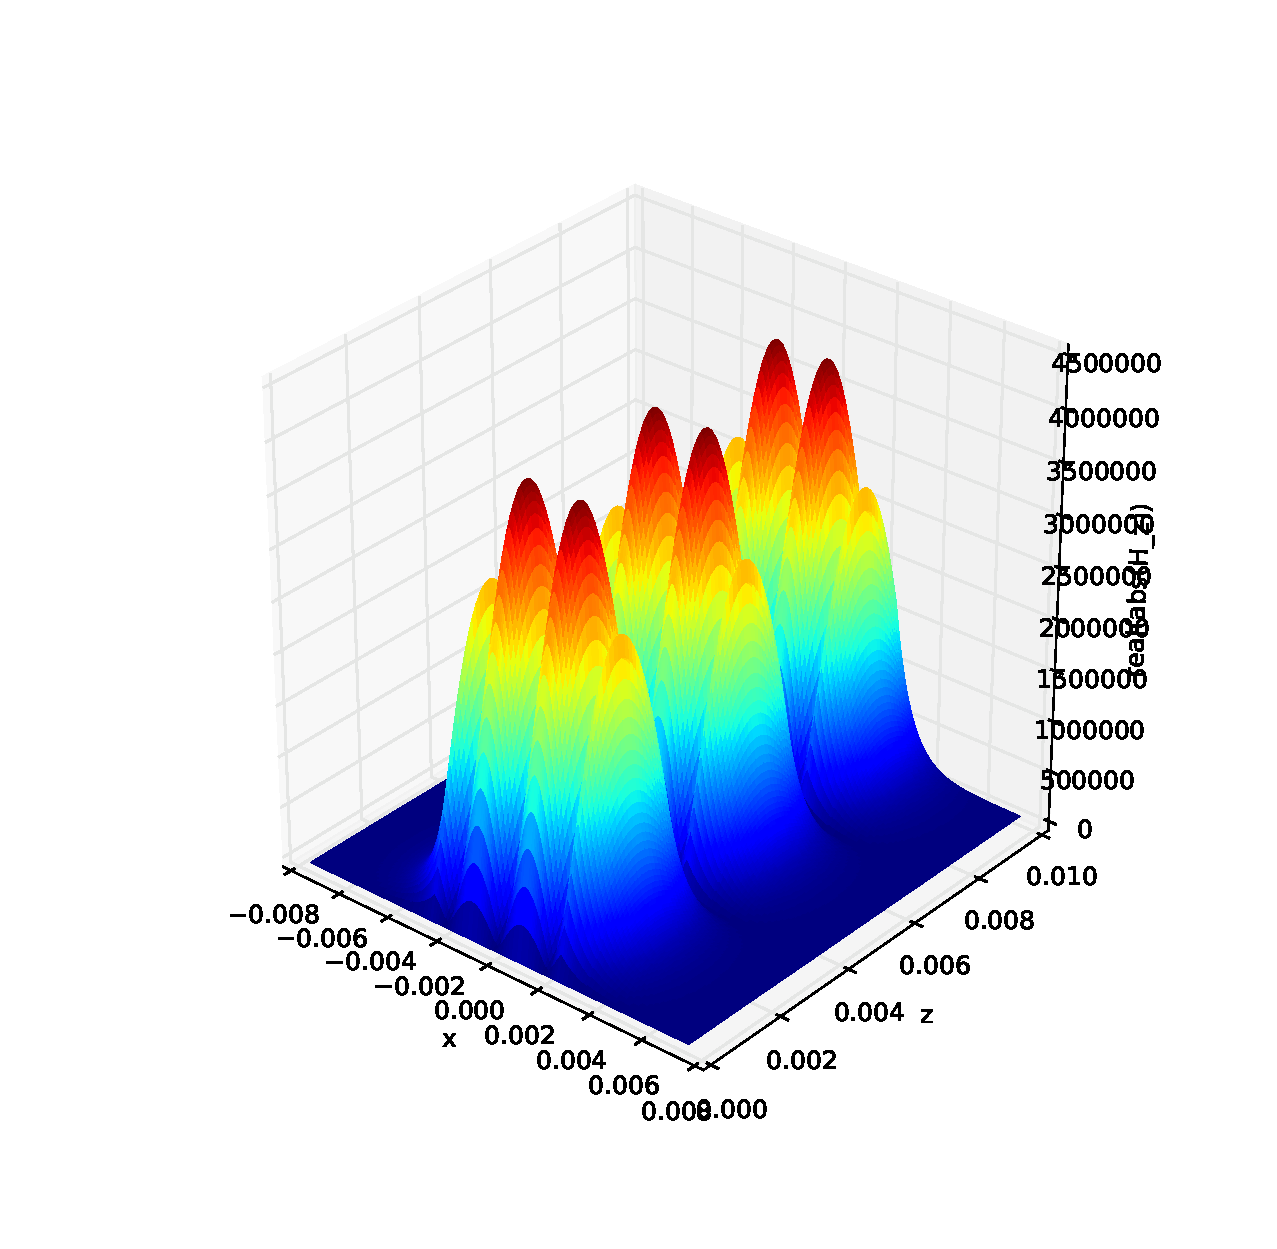
\includegraphics[width=1.5\textwidth]{H_z.pdf}}
  \caption{The figure depicts $|\Re(H_z(x,z,t))|$ at $\SI{50}{\giga\hertz}$ when the dielctric has a width of $\SI{5}{\milli\metre}$.}
  \label{fig:h_z}
\end{figure}
\begin{figure}
  \centering
  \noindent\makebox[\textwidth]{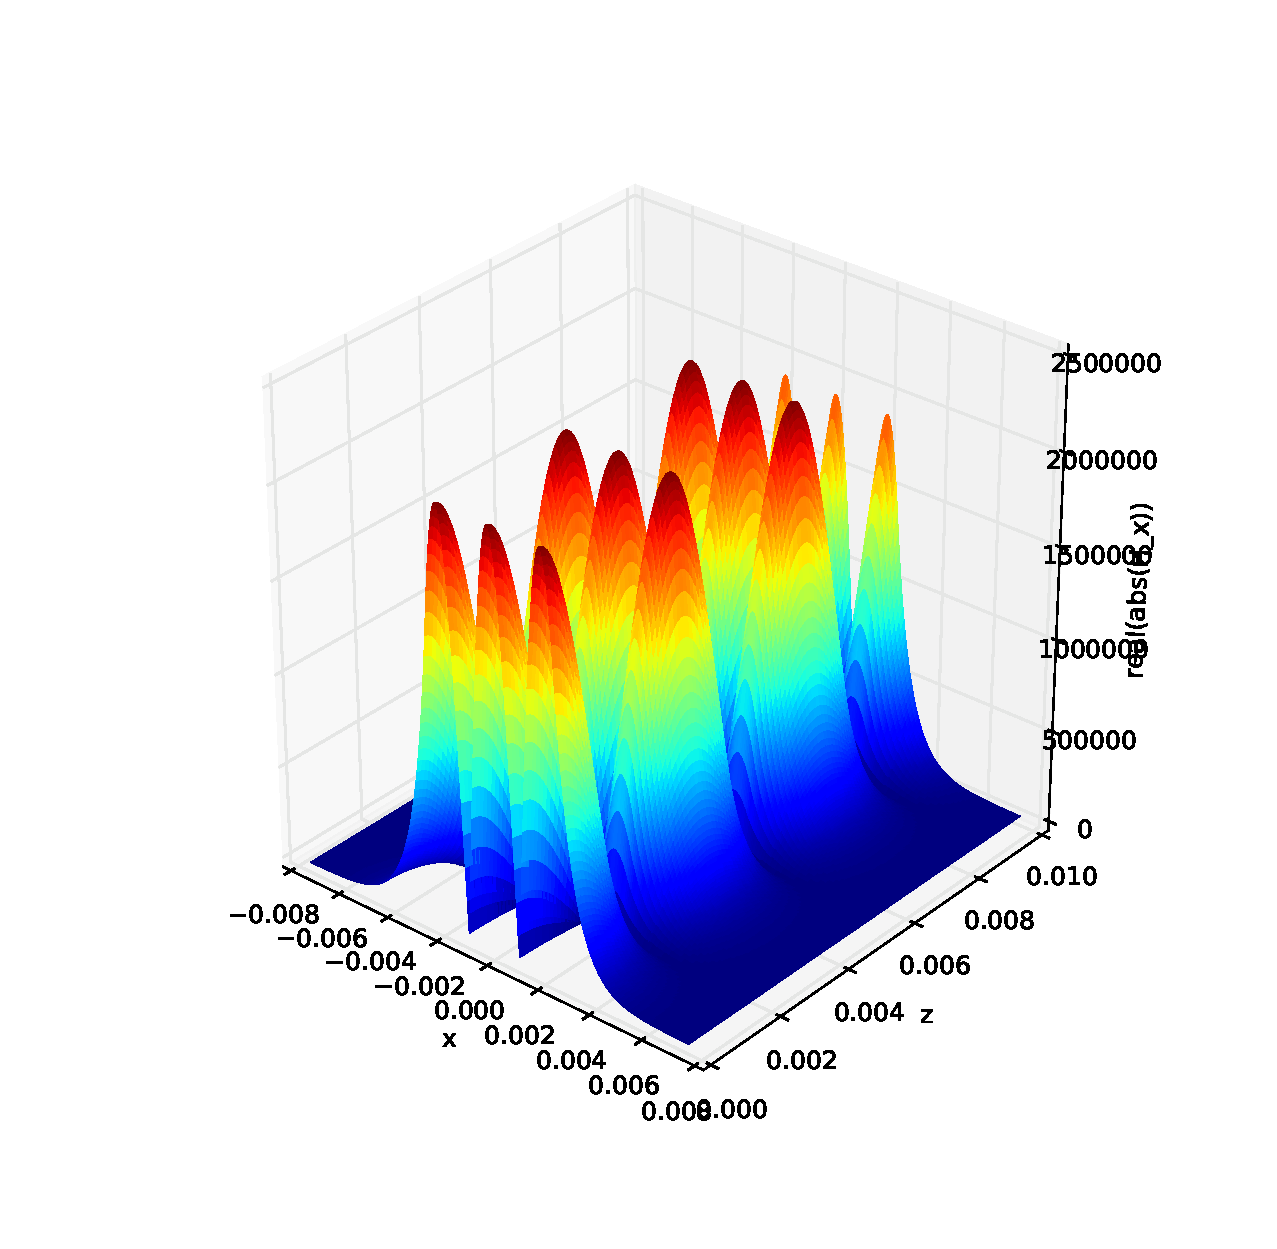
\includegraphics[width=1.5\textwidth]{H_x.pdf}}
  \caption{The figure depicts $|\Re(H_x(x,z,t))|$ at $\SI{50}{\giga\hertz}$ when the dielctric has a width of $\SI{5}{\milli\metre}$.}
  \label{fig:h_z}
\end{figure}
\begin{figure}
  \centering
  \noindent\makebox[\textwidth]{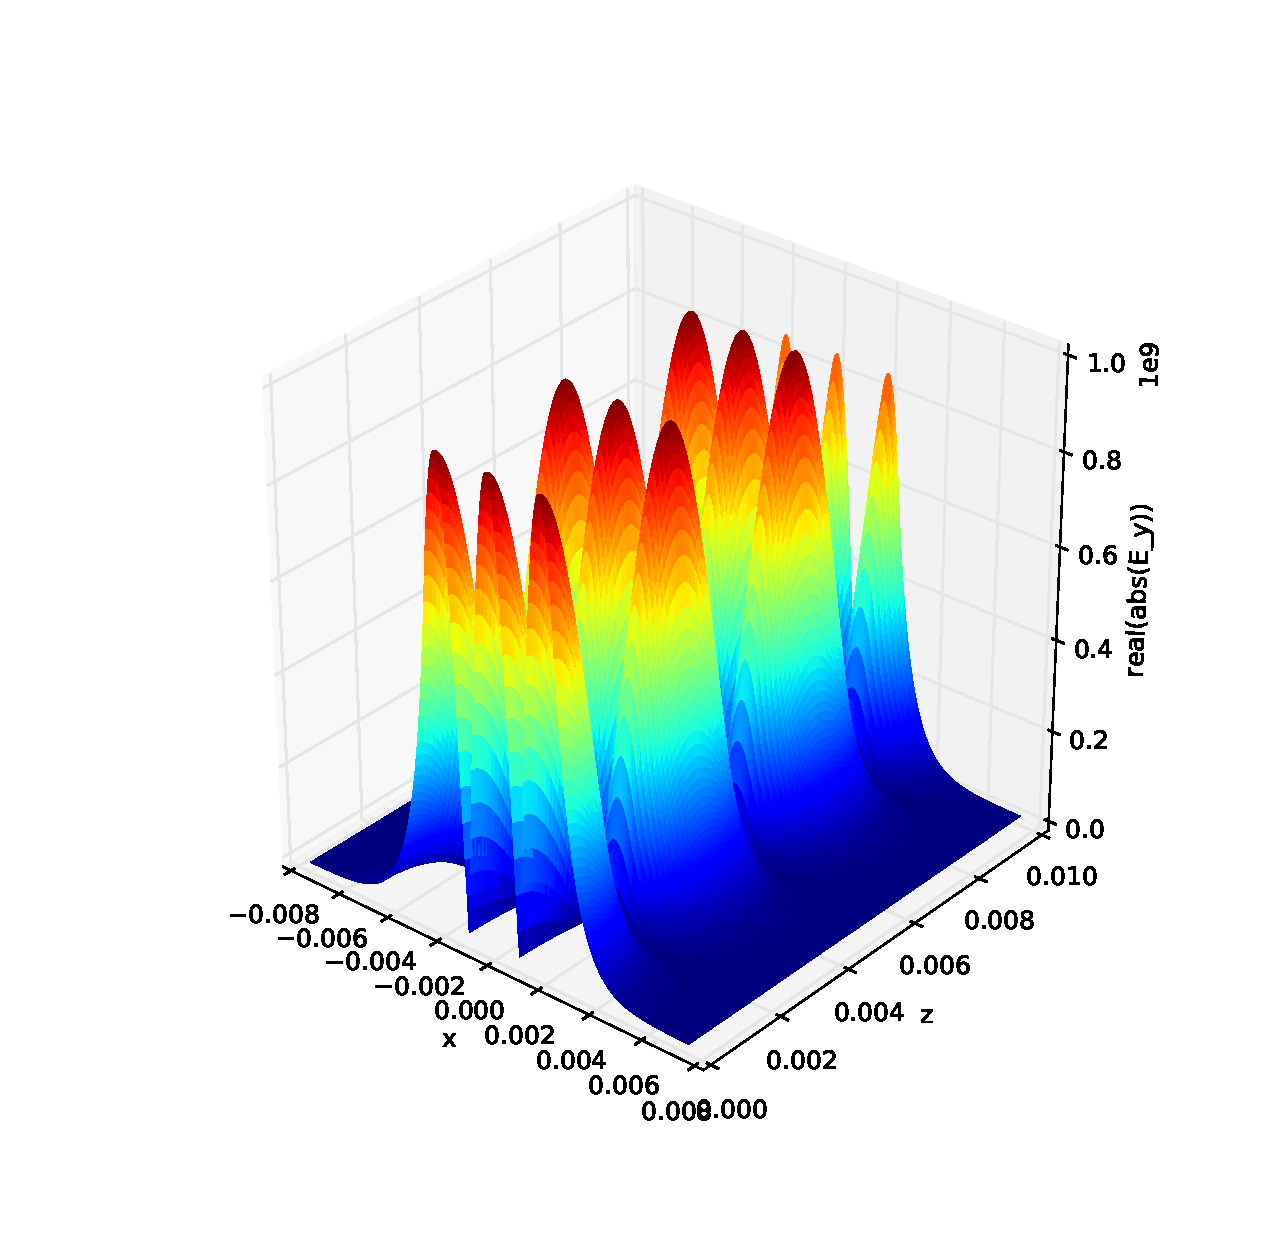
\includegraphics[width=1.5\textwidth]{E_y.pdf}}
  \caption{The figure depicts $|\Re(E_y(x,z,t))|$ at $\SI{50}{\giga\hertz}$ when the dielctric has a width of $\SI{5}{\milli\metre}$.}
  \label{fig:h_z}
\end{figure}

\subsection{c}\label{sec:c}
The cut-off frequency can be found from (\ref{eq:cutoff}) using appropriate values for the dielectric. The cut-off frequency is frequency dependent and is about $\SI{46.8}{\giga\hertz}$ for lower frequencies ($f \ll 10^{10}\SI{}{\hertz}$) and $\SI{34.6}{\giga\hertz}$ for higher frequencies ($f \gg 10^{10}\SI{}{\hertz}$). For the frequency at which the waveguide is designed for the cut-off frequency is $\SI{46.6}{\giga\hertz}$. Howerver, the wave starts to propagate at about $\SI{44.4}{\giga\hertz}$ which should be the ``true'' cut-off frequency.
\begin{equation}
  f_c = \dfrac{h}{2\pi\sqrt{\mu\epsilon}}
  \label{eq:cutoff}
\end{equation}


\subsection{d}\label{sec:d}
At $f=\SI{30}{\giga\hertz}$ the wave is evanescent since this frequency is below the cut-off frequency so it is not possible to create a $90^\text{o}$ section.

\subsection{e}\label{sec:d}

\subsection{f}\label{sec:d}
Magnetic walls are located where $\hat{n}\times\bar{H}=0$. While there are no complete magnetic walls there are ``walls'' where the current is several orders of magnitude lower than the peak values, which can bre seen in Figure~\ref{fig:magwall}.

\begin{figure}
  \centering
  \noindent\makebox[\textwidth]{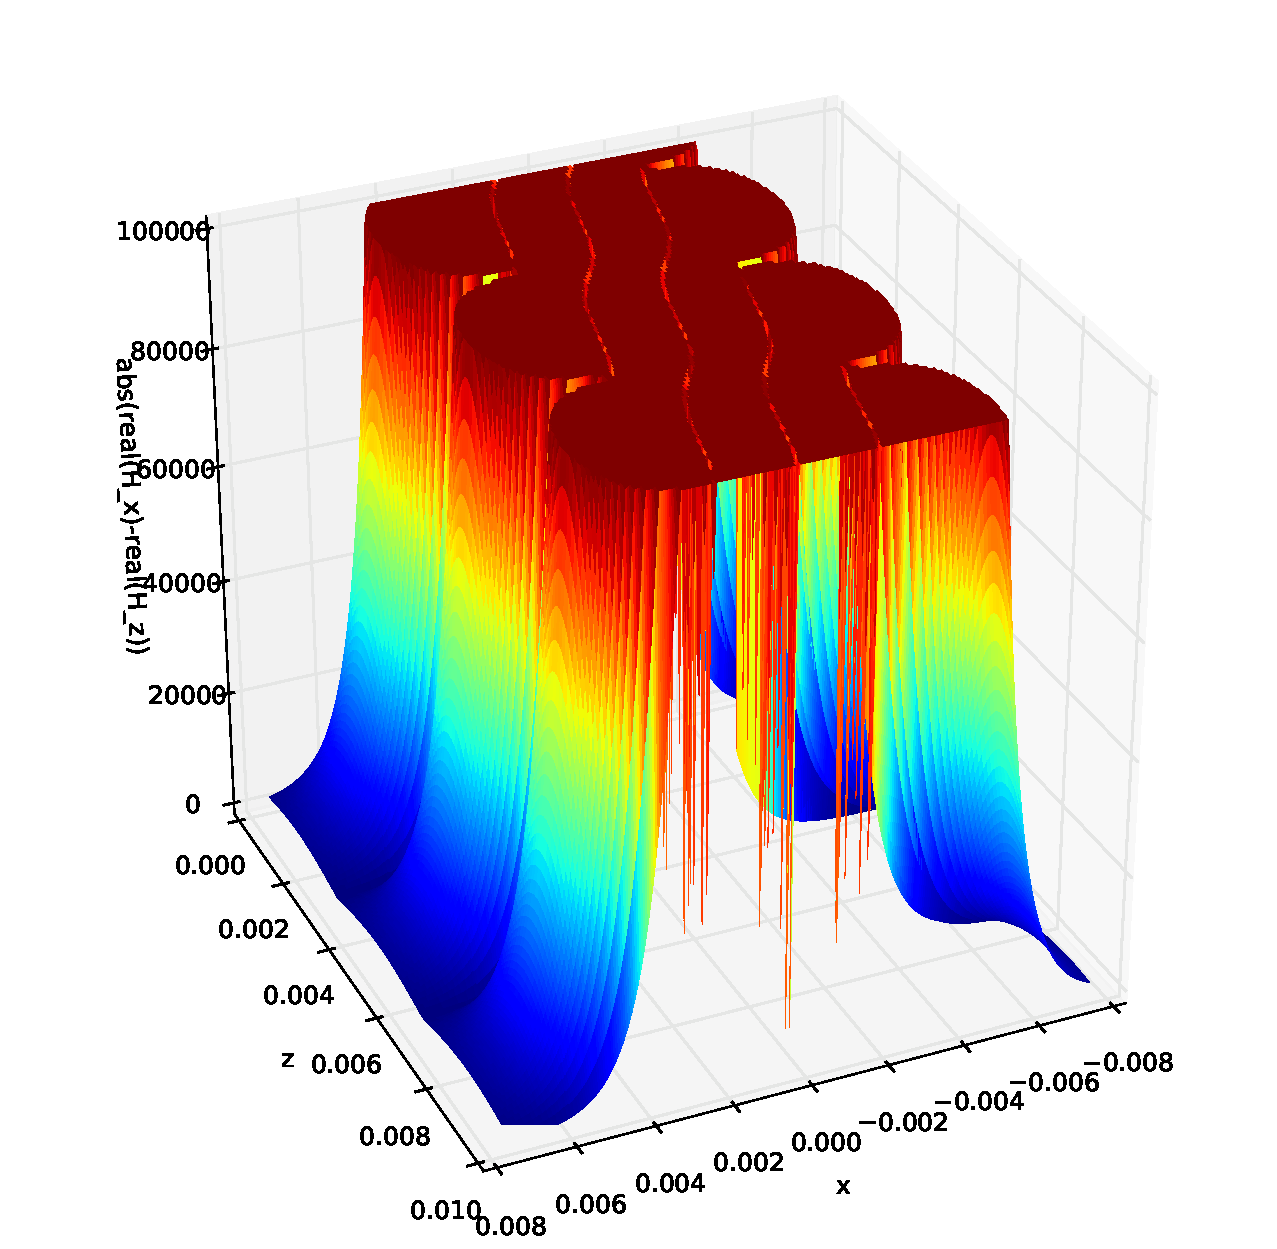
\includegraphics[width=1.5\textwidth]{mag_wall.pdf}}
  \caption{The figure depicts the magnitude of the current at $\SI{50}{giga\hertz}$ when the dielctric has a width of $\SI{5}{\milli\metre}$. There are parts where the current is several orders of magnitude lower than the peak values.}
  \label{fig:magwall}
\end{figure}

\end{document}